\section{Observation Processing}


The policy controls the agent's actions in the environment. The policy is optimized using the \ac{PPO} reinforcement learning algorithm. The policy takes a representation of the environment state as input and produces an action as output. This representation is called the observation.

The environment state is represented as an image from the agent's camera. This section explains how the observation is processed before it is given to the policy. The steps aim to enhance the policy's performance and generalization capabilities.

The agent's camera image has three channels, red, green, and blue. Its dimensions are defined by the config parameters $agentImageWidth$ and $agentImageHeight$. These parameters define the agent's field of view.
The policy receives an image from the agent camera as input. First the image is preprocessed. This changes the image content and dimensions. The preprocessed image is then combined with the memory mechanism to produce the inputs to the policy.


\subsection{Preprocessing}

The images from the agent camera are preprocessed before they are fed into the neural network. The preprocessing steps are applied to reduce the size of the neural network's input space. They are also applied to reduce the impact of different light settings on the policy's performance.
Three preprocessing steps have been implemented, downsampling, grayscale conversion, and histogram equalization. The preprocessing steps can be enabled and configured in the environment parameter $image\_preprocessing$. Each preprocessing step transforms an image into a new image. This can change the image dimensions and pixel domains. The steps are applied on the previous step's output. The steps are applied in order of downsampling, grayscale conversion, and histogram equalization. The first step takes the image from the agent camera as input.
The neural network uses the last step's output for inference.

The preprocessing steps are applied to all images from the agent camera. The table \ref{table:preprocessing_steps} shows how the preprocessing steps make images of different light settings more similar. The images in the table were generated using the configurations employed int the training runs.


\newcommand{\unityImg}[1]{\includegraphics[width=1\linewidth]{Bilder/image_printer_images/preprocessingSteps/fixedSpawnPoint_hardBlueFirstLeft_#1_image_from_unity.png}}
\newcommand{\downsampledImg}[1]{\includegraphics[width=1\linewidth]{Bilder/image_printer_images/preprocessingSteps/fixedSpawnPoint_hardBlueFirstLeft_#1_downsampled.png}}
\newcommand{\grayscaleImg}[1]{\includegraphics[width=1\linewidth]{Bilder/image_printer_images/preprocessingSteps/fixedSpawnPoint_hardBlueFirstLeft_#1_grayscale.png}}
\newcommand{\equalizedImg}[1]{\includegraphics[width=1\linewidth]{Bilder/image_printer_images/preprocessingSteps/fixedSpawnPoint_hardBlueFirstLeft_#1_equalized.png}}
\newcommand{\finalImg}[1]{\includegraphics[width=1\linewidth]{Bilder/image_printer_images/preprocessingSteps/fixedSpawnPoint_hardBlueFirstLeft_#1.png}}
\begin{table}
    \begin{center}
        \begin{tabular}{|| p{0.15\linewidth} || p{0.25\linewidth} | p{0.25\linewidth} | p{0.25\linewidth} ||}
            \hline
            light Setting                 & Bright                             & Standard                             & Dark                             \\ [0.5ex]
            \hline\hline
            Agent Camera Image from Unity & \makecell{\unityImg{bright}}       & \makecell{\unityImg{standard}}       & \makecell{\unityImg{dark}}       \\
            \hline
            Downsampled                   & \makecell{\downsampledImg{bright}} & \makecell{\downsampledImg{standard}} & \makecell{\downsampledImg{dark}} \\
            \hline
            Grayscale                     & \makecell{\grayscaleImg{bright}}   & \makecell{\grayscaleImg{standard}}   & \makecell{\grayscaleImg{dark}}   \\
            \hline
            Equalized                     & \makecell{\equalizedImg{bright}}   & \makecell{\equalizedImg{standard}}   & \makecell{\equalizedImg{dark}}   \\
            \hline
            Final Input Image             & \makecell{\finalImg{bright}}       & \makecell{\finalImg{standard}}       & \makecell{\finalImg{dark}}       \\
            \hline
        \end{tabular}
    \end{center}
    \caption{Preprocessing steps applied to images from the agent camera at the different light settings. The steps are applied in order from top to bottom.}
    \label{table:preprocessing_steps}
\end{table}

\subsubsection*{Benefits of reducing the input space size}

The reduction of input space size brings a variety of benefits. Some benefits are execution driven, like the reduction of the neural network's inference time. The neural network can make decisions quicker if it has to process fewer inputs. The reduction of the input space size also reduces the amount of data that has to be stored in memory. This is especially important during the training phase since many observations have to be stored in the rollout buffer.

The reduction of the input space size also reduces the number of parameters the neural network has to learn. This can lead to a more robust policy. Networks with smaller input spaces and less parameters are less prone to overfitting. The policy can generalize better to unseen situations.

% what datatype is used for the images? uint8? float32?
% there was a problem before with some datatype requiring more space than others
% change of datatype during preprocessing?

\subsubsection*{Benefits of reducing the impact of different light settings}

The policy has to be able to complete the different tracks for three different light settings. The policy is not provided with information about what light setting is active for the current episode. This means that the policy has to learn to produce correct actions for images of all three light settings. If images of the light settings look very different, the policy has to learn to the light settings as well as what action to take.
The preprocessing steps are applied to make images of different light settings more similar. The neural network is relieved of learning the different light settings. This can make learning easier and faster.
The preprocessing steps can also make the policy generalize better to unseen light settings. The policy can be trained on a single light setting and achieve good results for the other light setttings \ref{cha:experiment_fixed_difficulty_light_settings}.



\subsubsection{Downsampling}

The downsampling step changes the resolution and dimensions of the image. The step is configured with the $downsampling\_factor$ parameter. The downsampling factor is a positive integer and determines how much the image is downscaled. A $downsampling\_factor$ of one results in no downsampling. The width and height dimensions of the input image are divided by $downsampling\_factor$ to produce the new image dimensions.
The downsampling process divides the input image in a grid. The grid cells are $downsampling\_factor$ pixels wide and high. The pixel values of the new image are calculated by averaging the pixel values of the grid cells. The new image has a lower resolution than the input image.
Downsampling preserves the image content while reducing the size of the input space substantially.


\subsubsection{Grayscale}

The grayscale step converts the image to grayscale. The step can be enabled or disabled with the $grayscale$ parameter. The agent's camera image has three channels, red, green, and blue. The grayscale step changes the amount of channels and returns an image with a single grayscale channel. The grayscale image has the same width and height dimensions as the input image. The grayscaling reduces the input space size by a third.
The pixel values of the grayscale image are calculated as the weighted sum of intensities of the red, green, and blue channels. The weights are determined by the human eye's perception of the different colors. The grayscale value is computed as $Y = 0.2125 * R + 0.7154 * G + 0.0721 * B$.

The conversion to grayscale removes color information from the image. The alternating goal colors red and blue are no longer distinguishible. The advantage of grayscale images is that the policy's neural network does not have to learn the three dimensional colorspace of RGB images.



\subsubsection{Histogram Equalization}
\label{sec:histogram_equalization}

The histogram equalization step increases the contrast of the image. The step can be enabled or disabled with the $equalize\_histogram$ parameter. The histogram equalization step requires a grayscale image as input. The step changes the pixel values of the image. The step does not change the input space size.
The histogram equalization step changes the pixel values of the image. The histogram of the pixel intensities are made more uniform. First the cumulative histogram of the pixel intensities is calculated. The pixel values are then mapped to new values by using the cumulative histogram. The pixel values are distributed more evenly over the pixel value domain \ref{fig:histogram_equalization}.

The histogram equalization step can make images of different light settings more similar. The step also increases the contrast in the images. This can make it easier for the neural network to detect the objects.

\begin{figure}
    \centering
    \subfigure[Original Image]{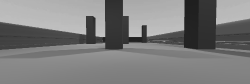
\includegraphics[width=0.3\textwidth]{Bilder/image_printer_images/histogram/original_image.png}}
    \subfigure[Equalized Image Image]{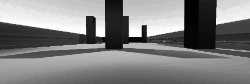
\includegraphics[width=0.3\textwidth]{Bilder/image_printer_images/histogram/equalized_image.png}}\\
    \subfigure[Original Image Histogram]{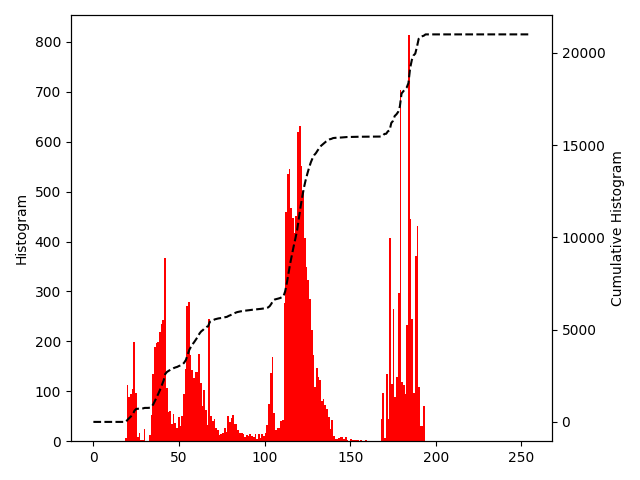
\includegraphics[width=0.3\textwidth]{Bilder/image_printer_images/histogram/original_histogram.png}}
    \subfigure[Equalized Image Histogram]{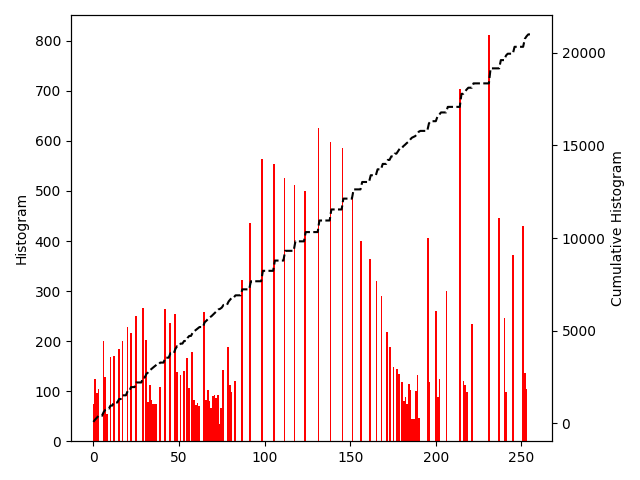
\includegraphics[width=0.3\textwidth]{Bilder/image_printer_images/histogram/equalized_histogram.png}}\\
    \caption{Histogram equalization of a grayscale image from standard light setting}
    \label{fig:histogram_equalization}
\end{figure}


\subsection{Memory Mechanism}

Memory mechanisms are a common approach to enhancing a reinforcement learning agent. Memory mechanisms can be implemented in many different ways. Our memory mechanism uses frame stacking, similar to \textcite{maximilian} and \textcite{atari}. The memory is configured with the $frame_stacking$ parameter. The memory is a simple first-in-first-out buffer that stores the last $frame_stacking$ images. The memory is updated by inserting the new image and removing the oldest image. The inserted images are the outputs of the preprocessing steps.
The images from the memory buffer are concatenated along the channel axis to produce the neural network input. This neural network input is essentially an image with many channels.
The memory buffer is reset at the start of every episode. The reset fills the entire buffer with zeros. The zeros are used as a placeholder. The first-in-first-out mechanism removes the zeros over the first $frame\_stacking$ timesteps.

The memory mechanism enables the policy to use information from previous time steps. The policy can use this information to detect objects that are not visible in the current image. Depending on the agent's position and orientation, the next goal might only be partially visible or not visible at all. The past images can help the policy reason about the next goal's position and how to continue.

% the memory also acts as a regularizer? more input data that can be used to learn the task? the images are highly correlated, it pobably would not need the newest image to decide on the action


\newcommand{\includePreprocessedImage}[1]{\includegraphics[width=0.15\textwidth]{Bilder/image_printer_images/memory_mechanism/preprocessed_image_step_#1.png}}
\newcommand\timestepT{5}
\newcommand\timestepTminusOne{4}
\newcommand\timestepTminusTwo{3}
\newcommand\timestepTminusThree{2}
\newcommand\timestepTminusFour{1}
\newcommand\imagesOffsetY{0}
\newcommand\inOutImageHeight{0.75}
\newcommand\bufferXOffset{-2}
\newcommand\bufferWidth{7}


\usetikzlibrary{fit}

\begin{figure}[!h]
    \centering
    \begin{tikzpicture}[%
            every node/.style={
                    font=\scriptsize,
                    % Better alignment, see https://tex.stackexchange.com/questions/315075
                    text height=1ex,
                    text depth=.25ex,
                },
        ]

        \node[inner sep=0pt] (newImg) at (-4,\inOutImageHeight)
        {\includePreprocessedImage{\timestepT}};
        \node[below] at (newImg.south) {New preprocessed image $t$};


        \node[inner sep=0pt] (step3) at (\bufferXOffset + 4.5,\imagesOffsetY + 1.5)
        {\includePreprocessedImage{\timestepTminusThree}};
        \node[below] at (step3.east) {image $t - 3$};

        \node[inner sep=0pt] (step2) at (\bufferXOffset + 3.5,\imagesOffsetY + 1)
        {\includePreprocessedImage{\timestepTminusTwo}};
        \node[below] at (step2.east) {image $t - 2$};

        \node[inner sep=0pt] (step1) at (\bufferXOffset + 2.5,\imagesOffsetY + 0.5)
        {\includePreprocessedImage{\timestepTminusOne}};
        \node[below] at (step1.east) {image $t - 1$};

        \node[inner sep=0pt] (step0) at (\bufferXOffset + 1.5,\imagesOffsetY)
        {\includePreprocessedImage{\timestepT}};
        \node[below] at (step0.south) {new image $t$};

        \node[fit={(\bufferXOffset,-0.55) (\bufferXOffset + \bufferWidth,2.5)}, inner sep=0pt, draw=blue, thick] (buffer) {};
        \node[below] (buffertext1) at (buffer.south) {Memory Buffer stack for timestep $t$};
        \node[below] (buffertext2) at (buffertext1.south) {$frame\_stacking = 4$};
        \node[below] (buffertext3) at (buffertext2.south) {Output dimensions: $[width, height, frame\_stacking]$};


        \node[inner sep=0pt] (outImg) at (7,\inOutImageHeight)
        {\includePreprocessedImage{\timestepTminusFour}};
        \node[below] at (outImg.south) {Removed image $t - 4$};

        \draw[->,thick] (\bufferXOffset - 0.75, 1) -- (\bufferXOffset, 1);
        \draw[->,thick] (\bufferXOffset + \bufferWidth, 1) -- (\bufferXOffset + \bufferWidth + 0.75, 1);


    \end{tikzpicture}
    \caption{Memory Mechanism}
    \label{fig:memory_mechanism}
\end{figure}